%Correct the file name.
%X: book number
%Y: part number
%ZZZ: page number in three digits. So page 3 would be 003.

\documentclass[11pt]{amsbook}

\usepackage{../HBSuerDemir}	% ------------------------


\begin{document}

% ++++++++++++++++++++++++++++++++++++++
\hPage{b2p1/031}
% ++++++++++++++++++++++++++++++++++++++

A series $\sum a_{n}$ such that $\sum|a_{n}|$ is convergent is called an
\\\underline{absolutely convergent series}, and the above theorem states \\that an absolutely convergent series is convergent.

As the alternating harmonic series shows, a series may be
\\convergent without being absolutely convergent. Such series are
\\called \underline{simply convergent}\footnote{In many textbooks \underline{conditional convergent} or \underline{semi-convergent} termi-
\\nologies are used instead of simply convergent.} series:
\begin{align*}
    \sum|a_{n}| \text{ (conv.)} 
        &\Longrightarrow \sum a_{n} \text{ (conv)} \dots \text{ abs. conv. of  } \sum a_{n}\\
    \sum|a_{n}| \text{ (div.)} 
        &\Longrightarrow \left\{
            \begin{array}{ll}
             \sum a_{n} \text{ (conv)} \dots \text{ simply. conv. of  } \sum a_{n}\\
             \text{or}\\
             \sum a_{n} \text{ (div)} 
    \end{array}
    \right.    
\end{align*}
There is an essential difference between the absolutely
\\convergent series and simply convergent ones. The absolutely conver-
\\gent series have the following two properties among others:

\begin{enumerate}
    \item The terms can be rearranged in any order (rearrangement does not alter the sum).
    \item Finitely or infinitely many terms may be replaced by their sum.
\end{enumerate}

These properties may not be shared by simply convergent 
\\series, that is, a rearrengement of terms in a simply convergent
\\series may give a different sum as illustrated by the following
\\example:

Consider the simply alternating harmonic series
\[
    S\:=\: 1 - \frac{1}{2} + \frac{1}{3} - \frac{1}{4} + \dots + (-1)^{n+1} \frac{1}{n} + \dots
\]

Let us rearrange the terms to have the series 

\[
    S'\:=\:(1-\frac{1}{2} - \frac{1}{4})+(\frac{1}{3} - \frac{1}{6} - \frac{1}{8}) +(\frac{1}{5} - \frac{1}{10} - \frac{1}{12})
\]
\[
    + \:\dots\:+\:(\frac{1}{2n+1} - \frac{1}{4n+2} -\frac{1}{4n+4} ) \:+\:\dots 
\]

% =======================================================
\end{document}  

%==== templates ====

%==== environments ====

%\begin{figure}[htb]
%	\centering
%	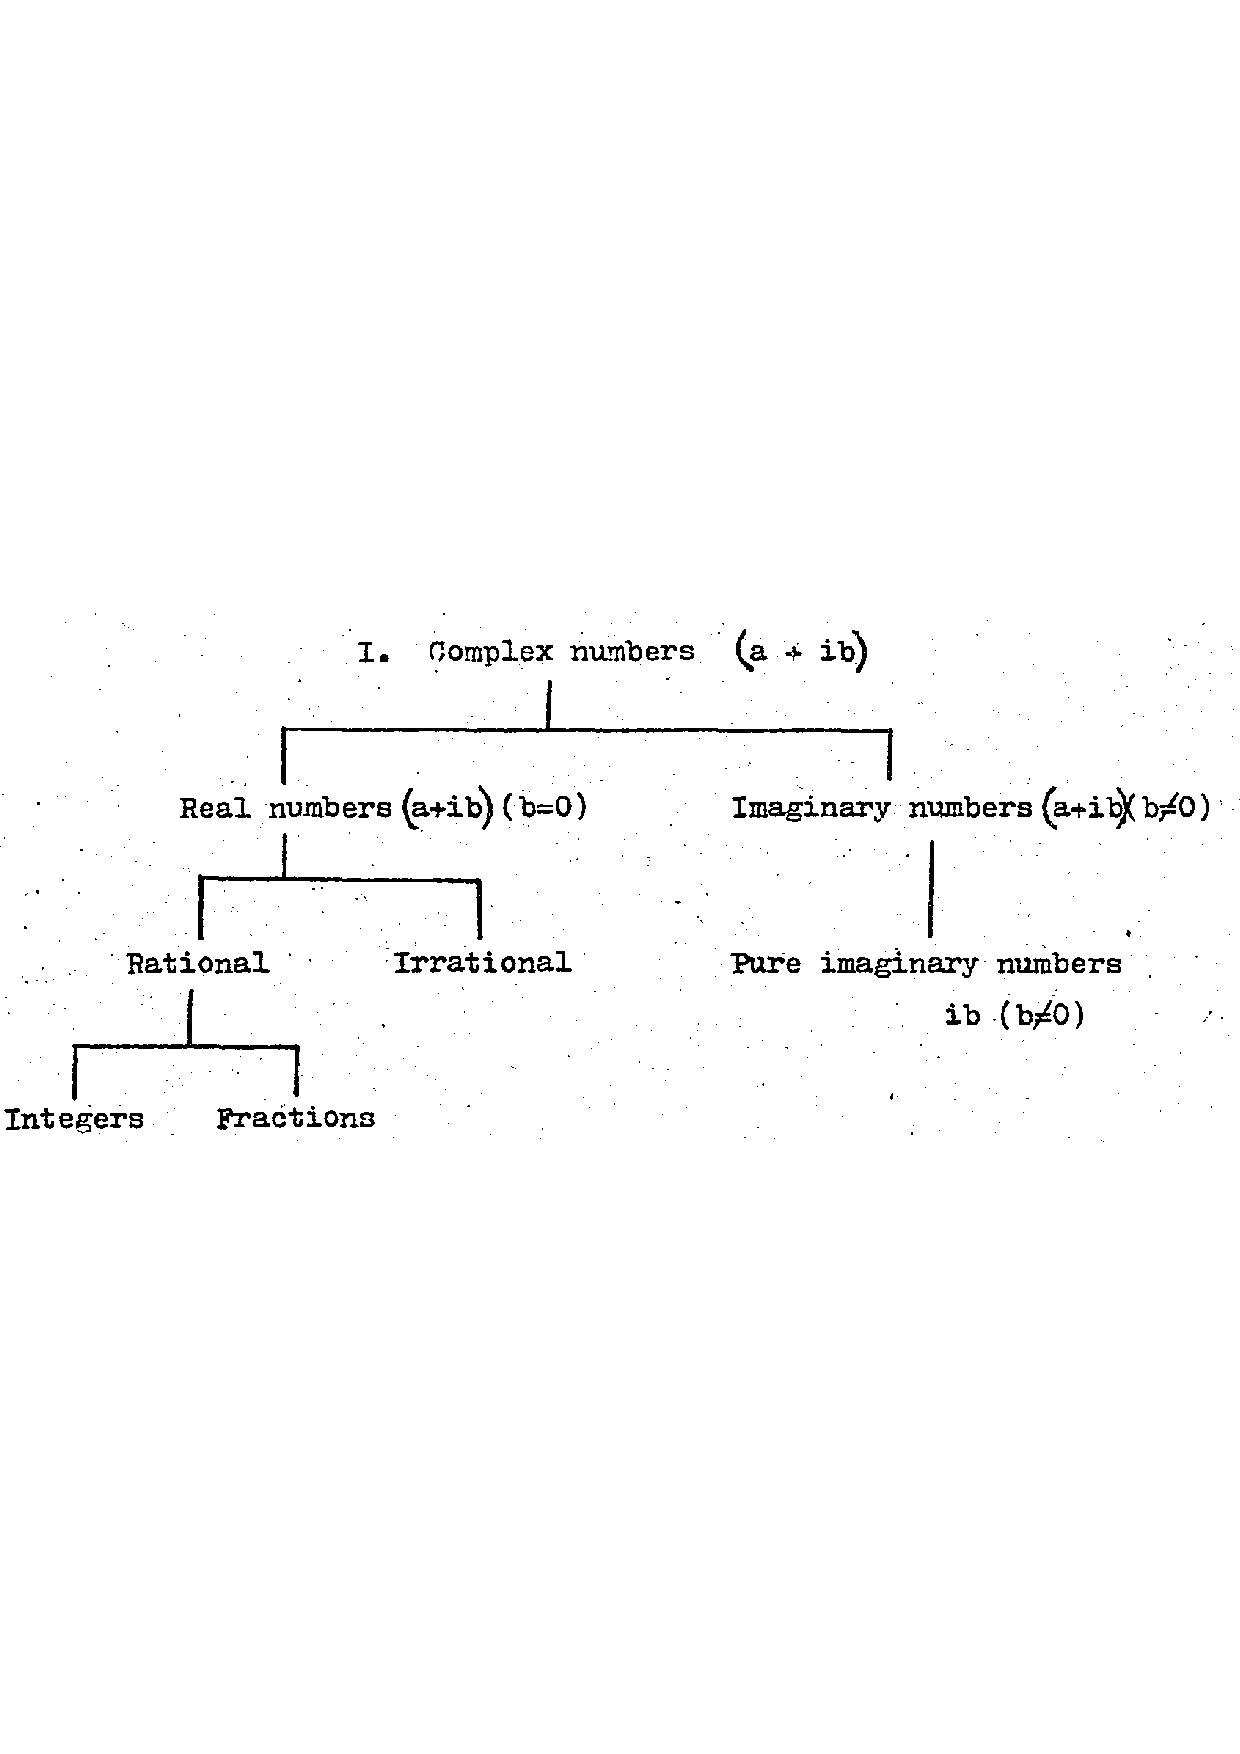
\includegraphics[width=0.9\textwidth]{images/SD-1-1p15A}
%	\caption{Classification of complex numbers}
%	\label{fig:classificationOfComplexNumbersA}
%\end{figure}

%\begin{center}
%\begin{tabular}{cc}
%\end{tabular}
%\end{center}

%\begin{exmp}
%\begin{hSolution}
%\end{hSolution}
%\end{exmp}

%\begin{hEnumerateAlpha}
%\end{hEnumerateAlpha}

%\begin{hEnumerateRoman}
%\end{hEnumerateRoman}

%$
%\begin{bmatrix}
%\end{bmatrix}
%$

%\frac{aaaa}{bbb}
%\frac{a_{n}}{b_{n}}
%\left( aaaa \right)
%\Longrightarrow

%\begin{multicols}{2}
%	bb
%\columnbreak
%	aa
%\end{multicols}
